\documentclass{article}

% Language setting
\usepackage[english]{babel}

% Set page size and margins
% Replace `letterpaper' with `a4paper' for UK/EU standard size
\usepackage[letterpaper,top=2cm,bottom=2cm,left=3cm,right=3cm,marginparwidth=1.75cm]{geometry}

% Useful packages
\usepackage{amsmath}
% --- Code listings ---
\usepackage{listings}
\usepackage{xcolor}
\definecolor{codegreen}{rgb}{0,0.6,0}
\definecolor{codegray}{rgb}{0.5,0.5,0.5}
\definecolor{codepurple}{rgb}{0.58,0,0.82}
\definecolor{backcolour}{rgb}{0.95,0.95,0.92}

\lstdefinestyle{mystyle}{
    backgroundcolor=\color{backcolour},   
    commentstyle=\color{codegreen},
    keywordstyle=\color{magenta},
    numberstyle=\tiny\color{codegray},
    stringstyle=\color{codepurple},
    basicstyle=\ttfamily\footnotesize,
    breakatwhitespace=false,         
    breaklines=true,                 
    captionpos=b,                    
    keepspaces=true,                 
    numbers=left,                    
    numbersep=5pt,                  
    showspaces=false,                
    showstringspaces=false,
    showtabs=false,                  
    tabsize=2
}

\lstset{style=mystyle}
% --- End Code Listings
\usepackage{graphicx}
\usepackage{float}
\usepackage{caption}
\captionsetup{labelformat=empty} 
% \usepackage{subcaption}
\usepackage[colorlinks=true, allcolors=blue]{hyperref}
\graphicspath{{./figures/}}

\title{ECE 637 Lab - Eigen-Decomposition of Images}
\author{Colin Braun}

\begin{document}
\maketitle

\stepcounter{section}
\section{Multivariate Gaussian Distributions and Whitening}
\subsection{Generating Gaussian Random Vectors}
\begin{figure}[H]
    \centering
    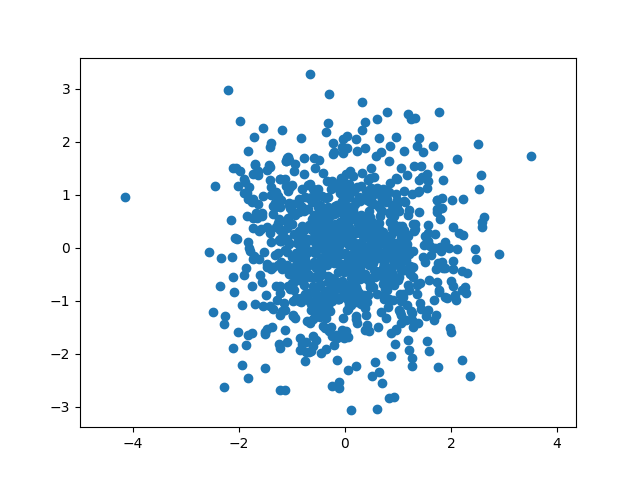
\includegraphics[width=1\textwidth]{../w-2-1.png}
        \end{figure}
\begin{figure}[H]
    \centering
    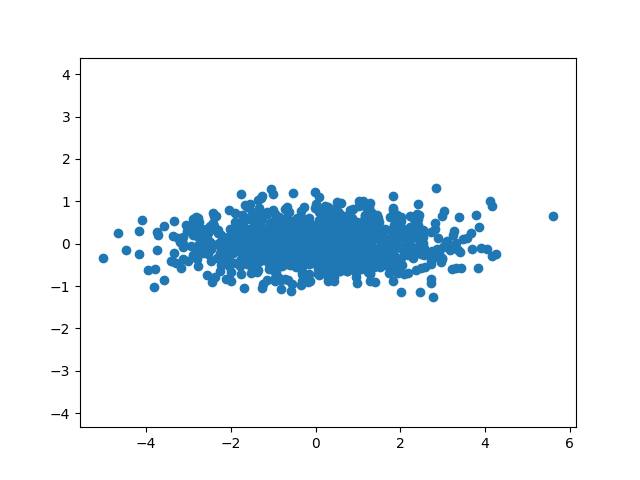
\includegraphics[width=1\textwidth]{../x-tilde-2-1.png}
        \end{figure}
\begin{figure}[H]
    \centering
    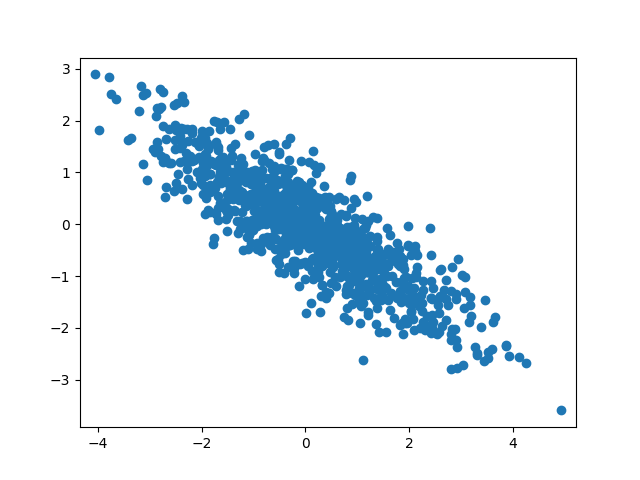
\includegraphics[width=1\textwidth]{../x-2-1.png}
        \end{figure}
\subsection{Covariance Estimation and Whitening}
The theoretical value of the covariance $R_x$ is given as
\begin{equation*}
R_x = 
\begin{bmatrix}
    2 & -1.2 \\
    -1.2 & 1
\end{bmatrix}
\end{equation*}.
The covariance estimate $\hat{R}_X$ is calculated to be
\begin{equation*}
\hat{R}_X = 
\begin{bmatrix}
    1.97 & -1.19 \\
    -1.19 & 0.99
\end{bmatrix}
\end{equation*}.
\begin{figure}[H]
    \centering
    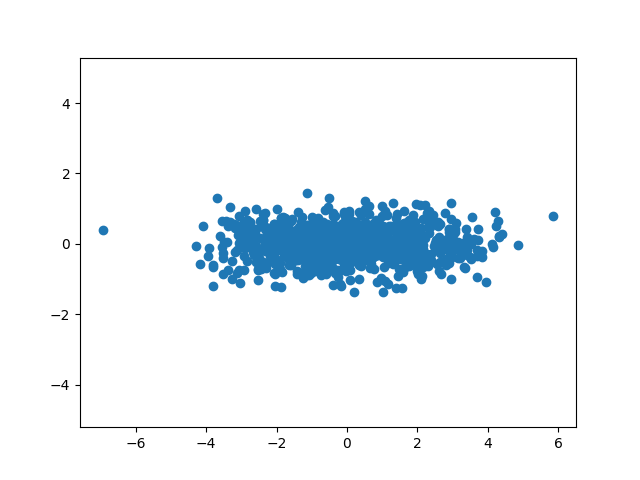
\includegraphics[width=1\textwidth]{../x-tilde-2-2.png}
        \end{figure}
\begin{figure}[H]
    \centering
    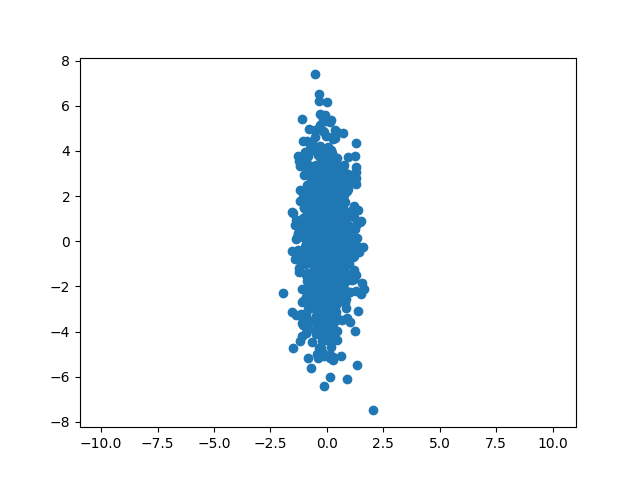
\includegraphics[width=1\textwidth]{../w-2-2.png}
\end{figure}
The covariance estimate $\hat{R}_W$ is calculated to be
\begin{equation*}
\hat{R}_W = 
\begin{bmatrix}
    0.34 & 0 \\
    0 & 4.87
\end{bmatrix}
\end{equation*}.

% Skip section 3
\stepcounter{section}
\section{Eigenimages, PCA, and Data Reduction}
\subsection{Exercise}
\begin{figure}[H]
    \centering
    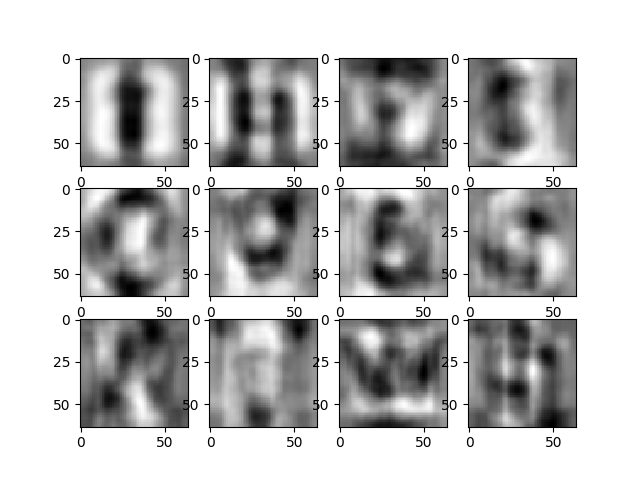
\includegraphics[width=1\textwidth]{../eigenimages.png}
\end{figure}
\begin{figure}[H]
    \centering
    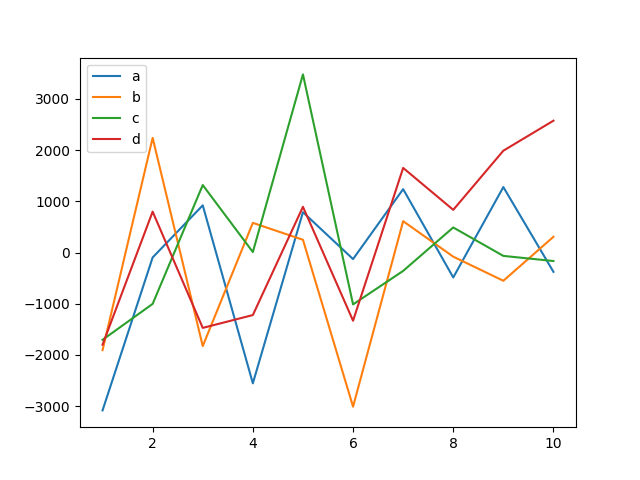
\includegraphics[width=1\textwidth]{../projection-coefficients.png}
\end{figure}
\begin{figure}[H]
    \centering
    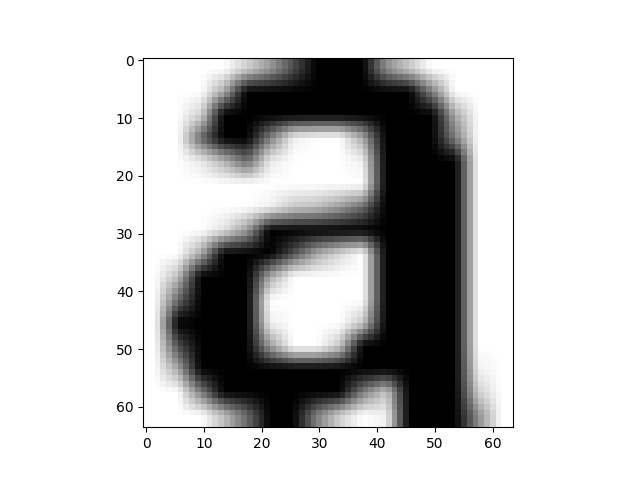
\includegraphics[width=1\textwidth]{../original-image.png}
\end{figure}

\section{Image Classification}
\subsection{Exercise: Classification and PCA}
\begin{table}[H]
    \centering
    \begin{tabular}{|c|c|}
        \hline
        Input Character & Classifier Output \\
        \hline
        d & a \\
        \hline
        j & y \\
        \hline
        l & i \\
        \hline
        n & v \\
        \hline
        p & e \\
        \hline
        q & a \\
        \hline
        u & a \\
        \hline
        y & v \\
        \hline
    \end{tabular}
    \caption{Mis-classified images using $R_k$}
\end{table}

\begin{table}[H]
    \centering
    \begin{tabular}{|c|c|}
        \hline
        Input Character & Classifier Output \\
        \hline
        i & l \\
        \hline
        y & v \\
        \hline
    \end{tabular}
    \caption{Mis-classified images using $B_k = \Lambda_k$}
\end{table}

\begin{table}[H]
    \centering
    \begin{tabular}{|c|c|}
        \hline
        Input Character & Classifier Output \\
        \hline
        g & q \\
        \hline
        y & v \\
        \hline
    \end{tabular}
    \caption{Mis-classified images using $B_k = R_{wc}$}
\end{table}

\begin{table}[H]
    \centering
    \begin{tabular}{|c|c|}
        \hline
        Input Character & Classifier Output \\
        \hline
        f & t \\
        \hline
        g & q \\
        \hline
    \end{tabular}
    \caption{Mis-classified images using $B_k = \Lambda$}
\end{table}

\begin{table}[H]
    \centering
    \begin{tabular}{|c|c|}
        \hline
        Input Character & Classifier Output \\
        \hline
        f & t \\
        \hline
        g & q \\
        \hline
        y & v \\
        \hline
    \end{tabular}
    \caption{Mis-classified images using $B_k = I$}
\end{table}

Clearly, among the above, the $B_k = \Lambda_k$, $B_k = R_{wc}$, and $B_k = \Lambda$ performed the best, only incorrectly classifying two characters.

TODO: Answer question 2

\end{document}
